% Hlavicka pro protokoly z fyzikalniho praktika.
% Verze pro: LaTeX
% Verze hlavicky: 22. 2. 2007
% Autor: Ustav fyziky kondenzovanych latek
% Ke stazeni: www.physics.muni.cz/ufkl/Vyuka/
% Licence: volne k pouziti, nejlepe k vcasnemu odevzdani protokolu z Vaseho mereni.


\documentclass[czech,11pt,a4paper]{article}
\usepackage[T1]{fontenc}
\usepackage{graphicx, animate}
\usepackage{mathtools}
\usepackage{amssymb}
\usepackage{amsthm}
\usepackage{thmtools}
\usepackage{xcolor}
\usepackage{nameref}
\usepackage{babel}
\usepackage{hyperref}
\usepackage{multicol}
\usepackage[export]{adjustbox}
\usepackage{subcaption}
\usepackage{caption}
\usepackage{multirow}
\usepackage{float}
\usepackage{placeins}
\graphicspath{ {./images/} }

\bibliographystyle{iso690}



%%% Nemente:
\usepackage[margin=2cm]{geometry}

%%% Nemente - konec.


%%%%%%%%%%% Doplnte pozadovane polozky:

%opening
\title{Využití ChatGPT v předmětu F2050 - Elektřina a magnetismus}
\author{Teodor Duraković}        
%%%%%%%%%%% Konec pozadovanych polozek.


%%%%%%%%%%% Uzitecne balicky:

%%%%%% Zamezeni parchantu:
\widowpenalty 10000 \clubpenalty 10000 \displaywidowpenalty 10000
%%%%%% Parametry pro moznost vsazeni vetsiho poctu obrazku na stranku
\setcounter{topnumber}{3}	  % max. pocet floatu nahore (specifikace t)
\setcounter{bottomnumber}{3}	  % max. pocet floatu dole (specifikace b)
\setcounter{totalnumber}{6}	  % max. pocet floatu na strance celkem
\renewcommand\topfraction{0.9}	  % max podil stranky pro floaty nahore
\renewcommand\bottomfraction{0.9} % max podil stranky pro floaty dole
\renewcommand\textfraction{0.1}	  % min podil stranky, ktery musi obsahovat text
\intextsep=8mm \textfloatsep=8mm  %\intextsep pro ulozeni [h] floatu a \textfloatsep pro [b] or [t]

% Tecky za cisly sekci:
\renewcommand{\thesection}{\arabic{section}.}
\renewcommand{\thesubsection}{\thesection\arabic{subsection}.}
\renewcommand{\thesubsubsection}{\thesubsection\arabic{subsubsection}.}
% Jednopismenna mezera mezi cislem a nazvem kapitoly:
\makeatletter \def\@seccntformat#1{\csname the#1\endcsname\hspace{1ex}} \makeatother


%%%%%%%%%%%%%%%%%%%%%%%%%%%%%%%%%%%%%%%%%%%%%%%%%%%%%%%%%%%%%%%%%%%%%%%%%%%%%%%
%%%%%%%%%%%%%%%%%%%%%%%%%%%%%%%%%%%%%%%%%%%%%%%%%%%%%%%%%%%%%%%%%%%%%%%%%%%%%%%
% Zacatek dokumentu
%%%%%%%%%%%%%%%%%%%%%%%%%%%%%%%%%%%%%%%%%%%%%%%%%%%%%%%%%%%%%%%%%%%%%%%%%%%%%%%
%%%%%%%%%%%%%%%%%%%%%%%%%%%%%%%%%%%%%%%%%%%%%%%%%%%%%%%%%%%%%%%%%%%%%%%%%%%%%%%

\begin{document}
	
	%%%%%%%%%%%%%%%%%%%%%%%%%%%%%%%%%%%%%%%%%%%%%%%%%%%%%%%%%%%%%%%%%%%%%%%%%%%%%%%
	% Nemente:
	%%%%%%%%%%%%%%%%%%%%%%%%%%%%%%%%%%%%%%%%%%%%%%%%%%%%%%%%%%%%%%%%%%%%%%%%%%%%%%%

	
	

	\maketitle

		
	
	
	\vskip1cm
	
	%%%%%%%%%%%%%%%%%%%%%%%%%%%%%%%%%%%%%%%%%%%%%%%%%%%%%%%%%%%%%%%%%%%%%%%%%%%%%%%
	% konec Nemente.
	%%%%%%%%%%%%%%%%%%%%%%%%%%%%%%%%%%%%%%%%%%%%%%%%%%%%%%%%%%%%%%%%%%%%%%%%%%%%%%%
	
	%%%%%%%%%%%%%%%%%%%%%%%%%%%%%%%%%%%%%%%%%%%%%%%%%%%%%%%%%%%%%%%%%%%%%%%%%%%%%%%
	%%%%%%%%%%%%%%%%%%%%%%%%%%%%%%%%%%%%%%%%%%%%%%%%%%%%%%%%%%%%%%%%%%%%%%%%%%%%%%%
	% Zacatek textu vlastniho protokolu
	%%%%%%%%%%%%%%%%%%%%%%%%%%%%%%%%%%%%%%%%%%%%%%%%%%%%%%%%%%%%%%%%%%%%%%%%%%%%%%%
	%%%%%%%%%%%%%%%%%%%%%%%%%%%%%%%%%%%%%%%%%%%%%%%%%%%%%%%%%%%%%%%%%%%%%%%%%%%%%%%
	
	\begin{multicols}{2}
		\begin{abstract}
			Generativní velké jazykové modely (angl. LLM) se v době psaní textu již dostaly na úroveň, kdy dokáží bez větší asistence uživatele řešit složitější problémy. V této práci budeme zkoumat schopnost různých jazykových modelů řešit úlohy používané v základním kurzu fyziky pojednávajícím o elektřině a magnetismu - ten se k této práci hodí i proto, že obtížnost látky v něm probírané postupně roste - od základních diferenciálních operátorů až po vícerozměrnou integraci s transformovanými souřadnicemi. Předpokládáme, že výsledky budou spolehlivě demonstrovat samostatnost novějších modelů, u modelů starších naopak očekáváme větší chybovost a nižší schopnost řešení složitějších problémů. 
		\end{abstract}
		\section{Metodika}
		Ze sbírky \cite{cviceni} je vybráno dvacet úloh pokrývajících látku celého kurzu, ty jsou zpracovány ChatGPT \cite{ChatGPT}, konkrétně modely o1, o3-mini, GPT-4, GPT-4o mini, GPT-4o a GPT-4.5, modely Grok 2 a Grok 3 od xAI\cite{Grok} a Claude 3.7 od Anthropic\cite{Claude}. U modelů, kde to je možné (ChatGPT, Grok), je použita funkce \textit{temporary chat}, při které není využívána lokální paměť jazykového modelu a komunikace není využita k dalšímu trénování modelů. Claude dle dostupných informací data k trénování nevyužívá\cite{anthropicprivacy}. \\V instrukci je podáno pouze zadání bez jiných doplnění, případná matematická notace je v instrukci formulována ve standardní sazbě jazyku LaTeX, jelikož veškeré modely tuto sazbu, případně její deriváty, využívají. Za správnou odpověď je zaznamenán 1 bod, při nesprávné odpovědi je model o chybě informován bez bližší specifikace chyby. Je-li při druhém pokusu odpověď správná, je uděleno 0.5 bodu. Dále je hodnocen způsob komunikace - na škále 0.1-1 bodů hodnotíme kvalitu odpovědi, veškerá zdůvodnění a postupy. Plný bod získává odpověď správně vysvětlující celé řešení jednoduchým způsobem bez zbytečných komplikací - bez jakéhokoliv cíleného ladění instrukcí (tzv. prompt-engineeringu) od chatbotů předpokládáme odpověď delší, vysvětlující použité principy. Zbytečně složitý postup je stejně jako výsledek bez vysvětlení důvodem pro nižší ohodnocení. V hodnocení tohoto kritéria vycházíme ze základního předpokladu naší práce - hodnotíme právě to, jak LLM dokáží řešit úlohy vyskytující se v daném předmětu a uživateli s řešením problémů asistovat. Posledním hodnoceným faktorem je rychlost. Zde se snažíme zamezit vnějším vlivům, jako je kupř. fluktuace rychlosti internetu. Danou otázku tedy postupně bez zbytečných přestávek pokládáme všem modelům v systému, v takto malém časovém okně lze totiž předpokládat, že se rychlost síťové komunikace zásadně nezměnila. Během měření se snažíme udržovat zátěž využívaného počítače konstantní, aby ani tento faktor rychlost neovlivňoval. \\
		Zde je důležité konstatovat, že neměříme čistou rychlost fungování jednotlivých modelů - výsledná rychlost je kombinací výkonu modelu, kvality připojení, rychlosti serveru a dalšími parametry, které nejsou závislé na samotném modelu, ale konkrétním serveru, jeho optimalizaci a zatížení. Pro účely naší práce tyto rychlosti není nutné separovat - pro koncového uživatele je důležitá právě rychlost celková. Zde jistým zjednodušením předpokládáme, že je relativní zátěž konkrétních serverů v daný čas stejná \footnote{Celý experiment byl proveden až po velikém nárazovém nárůstu uživatelů služeb OpenAI spjatým s neobvykle vysokou zátěží\cite{ET2025ghibli}. Předpokládáme, že v době provedení experimentu byly servery již vytížené obvyklou intenzitou.} - nemožnost tuto metriku analyzovat nám jiný postup ani neumožňuje.
		\newpage
		\section{Výsledky a zpracování dat}
		Při výše uvedeném postupu jsme získali výsledky uvedené na tab. 1.
	\end{multicols}
		\begin{table}[H]
			\centering

				{\scriptsize \begin{tabular}{l|lll|lll|lll|lll|lll}
					\hline
					model &  1-z &  1-r &    1-t &  2-z &  2-r &    2-t &  3-z &  3-r &    3-t &  4-z &  4-r &    4-t &  5-z &  5-r &    5-t \\ \hline
					
					
					o1 &           1 &              1 &  12.75 &           1 &              1 &  52.52 &           1 &              1 &  17.92 &           1 &            0.1 &  12.54 &           1 &              1 &   24.3 \\
					o3-mini &           1 &              1 &  24.63 &           1 &            0.1 &  81.89 &           1 &            0.1 &  38.62 &           1 &              1 &  28.89 &           1 &              1 &  33.74 \\
					4 &           1 &            0.1 &  61.88 &           1 &              1 &  71.44 &           0 &              0 &     90 &           1 &            0.1 &  42.64 &           1 &              1 &  67.06 \\
					4o-mini &           1 &              1 &  48.54 &           1 &              1 &  81.61 &           1 &            0.1 &  39.18 &           1 &              1 &  33.88 &           1 &              1 &  27.38 \\
					4o  &           1 &              1 &  39.06 &           1 &              1 &  50.34 &           1 &              1 &   25.6 &           1 &              1 &  33.24 &           1 &              1 &  25.56 \\
					4.5 &           1 &              1 &   33.9 &           1 &              1 &  79.17 &           1 &              1 &  39.39 &           1 &              1 &  54.07 &           1 &              1 &  54.09 \\
					Grok 2 &           1 &              1 &  20.65 &           1 &              1 &  28.21 &           0 &              0 &  41.59 &           1 &            0.8 &  21.24 &           1 &              1 &  23.54 \\
					Grok 3 &           1 &              1 &   15.1 &           1 &            0.8 &  29.82 &           0 &              0 &  34.32 &           1 &              1 &  21.25 &           1 &              1 &  26.29 \\
					Claude 3.7 Sonnet &           1 &              1 &  21.51 &           1 &            0.8 &  51.09 &           1 &              1 &  27.98 &           1 &              1 &  26.71 &           1 &              1 &  22.16 \\ \hline 
					model &  6-z &  6-r &    6-t &  7-z &  7-r &    7-t &  8-z &  8-r &    8-t &  9-z &  9-r &    9-t & 10-z & 10-r &   10-t \\ \hline
					o1 &           1 &              1 &  77.44 &           1 &            0.1 & 110.25 &           1 &              1 &  24.79 &           1 &              1 & 116.78 &           1 &            0.1 &  37.24 \\
					o3-mini &           1 &              1 &  59.92 &           1 &              1 & 128.06 &           1 &              1 &  37.06 &           1 &              1 &    104 &           1 &            0.1 &     31 \\
					4 &           1 &              1 &     63 &           0 &              0 &    200 &           1 &              1 &  55.96 &           1 &              1 &  63.53 &           1 &              1 &   46.4 \\
					4o-mini &           1 &              1 &  25.21 &           0 &              0 &    141 &           1 &            0.1 &  35.49 &           0 &              0 &  83.58 &           1 &            0.1 &  26.54 \\
					4o  &           1 &            0.1 &  99.13 &           1 &              1 &  51.46 &           1 &              1 &  36.44 &           1 &              1 &   68.7 &           1 &              1 &  57.54 \\
					4.5 &           1 &              1 & 121.26 &           1 &              1 &    130 &           1 &              1 &  59.24 &           1 &              1 &   94.6 &           1 &              1 &  50.29 \\
					Grok 2 &           1 &            0.1 &  27.06 &           1 &            0.2 &   40.6 &           1 &              1 &  31.42 &           1 &            0.8 &  37.02 &           1 &              1 &  29.32 \\
					Grok 3 &           1 &            0.4 &  36.23 &           1 &            0.4 &   40.8 &           1 &            0.8 &  25.36 &           1 &            0.6 &  40.23 &           1 &            0.8 &  19.27 \\
					Claude 3.7 Sonnet &           1 &              1 &  39.31 &           1 &            0.6 &  52.04 &           1 &            0.2 &  34.77 &           1 &            0.7 &     60 &           1 &              1 &  28.64 \\ \hline 
					model & 11-z & 11-r &   11-t & 12-z & 12-r &   12-t & 13-z & 13-r &   13-t & 14-z & 14-r &   14-t & 15-z & 15-r &   15-t \\ \hline
					o1 &           1 &              1 &  33.88 &           1 &            0.1 &  23.41 &           1 &            0.1 &  23.36 &           1 &            0.5 &  83.75 &           1 &            0.1 &   9.59 \\
					o3-mini &           1 &              1 &   52.3 &           1 &              1 &  81.97 &           1 &              1 &  29.82 &           1 &              1 &  74.51 &           1 &            0.5 &  25.51 \\
					4 &           1 &              1 &  49.99 &           1 &              1 &  59.75 &           1 &            0.1 &  63.72 &           1 &            0.5 &  56.86 &           1 &            0.5 &  49.89 \\
					4o-mini &           1 &            0.1 &  38.01 &           1 &            0.1 &  21.93 &           1 &              1 &   28.9 &           0 &              0 &     79 &           1 &            0.5 &  15.75 \\
					4o  &           1 &              1 &   62.1 &           1 &            0.1 &  62.34 &           1 &              1 &   29.1 &           1 &              1 &  63.84 &           1 &            0.5 &  35.55 \\
					4.5 &           1 &              1 &     62 &           1 &            0.5 & 102.19 &           1 &              1 &  63.71 &           1 &              1 & 104.36 &           1 &              1 &  51.25 \\
					Grok 2 &           1 &            0.8 &  33.64 &           1 &            0.1 &  38.45 &           1 &            0.8 &  32.24 &           1 &            0.5 &  43.03 &           1 &            0.5 &  24.99 \\
					Grok 3 &           1 &              1 &   23.2 &           1 &            0.1 &   38.5 &           1 &              1 &  25.79 &           1 &            0.1 &  76.79 &           1 &            0.5 &  26.87 \\ 
					Claude 3.7 Sonnet &           1 &            0.1 &  41.63 &           0 &              0 &  46.88 &           1 &              1 &  27.14 &           1 &            0.5 &  36.83 &           1 &            0.5 &   10.3 \\ \hline 
					model & 16-z & 16-r &   16-t & 17-z & 17-r &   17-t & 18-z & 18-r &   18-t & 19-z & 19-r &   19-t & 20-z & 20-r &   20-t \\ \hline
					o1 &           1 &            0.1 &  10.67 &           1 &            0.8 & 109.07 &           1 &              1 &  36.02 &           1 &              1 &   12.1 &           1 &              1 &  42.79 \\
					o3-mini &           1 &              1 &   51.2 &           1 &            0.6 &  64.52 &           1 &              1 &  34.01 &           1 &              1 &  14.52 &           1 &              1 &  90.15 \\
					4 &           1 &            0.1 &     40 &           1 &            0.2 &  93.28 &           0 &              0 & 102.25 &           1 &              1 &  42.63 &           0 &              0 &     90 \\
					4o-mini &           1 &            0.5 &  25.46 &           1 &            0.8 &  51.02 &           0 &              0 &  44.43 &           1 &              1 &  18.36 &           0 &              0 &  48.79 \\
					4o  &           1 &            0.8 &  33.55 &           1 &              1 &  59.15 &           1 &              1 &  31.64 &           1 &              1 &  19.25 &           1 &              1 &  51.23 \\
					4.5 &           1 &              1 &  64.06 &           1 &              1 &  117.6 &           1 &            0.8 & 168.42 &           1 &              1 &  62.53 &           1 &            0.4 & 115.66 \\
					Grok 2 &           1 &            0.8 &   32.6 &           1 &            0.2 &  42.17 &           0 &              0 &  28.86 &           1 &            0.8 &  14.17 &         0.5 &            0.4 &  75.25 \\
					Grok 3 &           1 &            0.5 &   38.6 &           1 &              1 &  35.55 &           1 &            0.1 &  30.08 &           1 &              1 &  17.76 &           0 &              0 &  61.91 \\
					Claude 3.7 Sonnet &           1 &            0.5 &  20.51 &           1 &              1 &  35.22 &           1 &              1 &  24.39 &           1 &              1 &  19.51 &           1 &              1 &  32.55 \\
				\end{tabular}}
				
				
				\caption{Výsledek měření - tři hodnocené faktory jsou v tabulce zastoupeny písmenem z pro správnost (původně známka), r pro kvalitu komunikace (reasoning) a t pro čas v sekundách(time).}
			\end{table}
		\begin{multicols}{2}
		Pro přehledné zpracování výsledků je měřený čas upraven následovně: jelikož pro nás má větší výpovědní hodnotu čas relativní, nikoliv absolutní, normujeme jej podle nejrychlejšího z modelů. Nejnižší průměrný čas má model Claude 3.7 Sonnet s $\overline{t_C} = 32.96\,\mathrm{s}$ Pro každou otázku je čas zmíněného modelu brán jako referenční a hodnoty jsou transformovány formulí $T = \frac{{t_c}}{t}$, čímž znovu dostaneme výsledky s většinou hodnot v intervalu (0,1) - v situacích, kdy je rychlejší jiný model než referenční, získáme hodnotu větší než 1. Stejně jako u ostatních hodnocených kritérií však platí, že větší hodnota znamená lepší výsledek. Zpracováním těchto dat lze modely vzájemně srovnat:
		\begin{figure}[H]
			\centering
			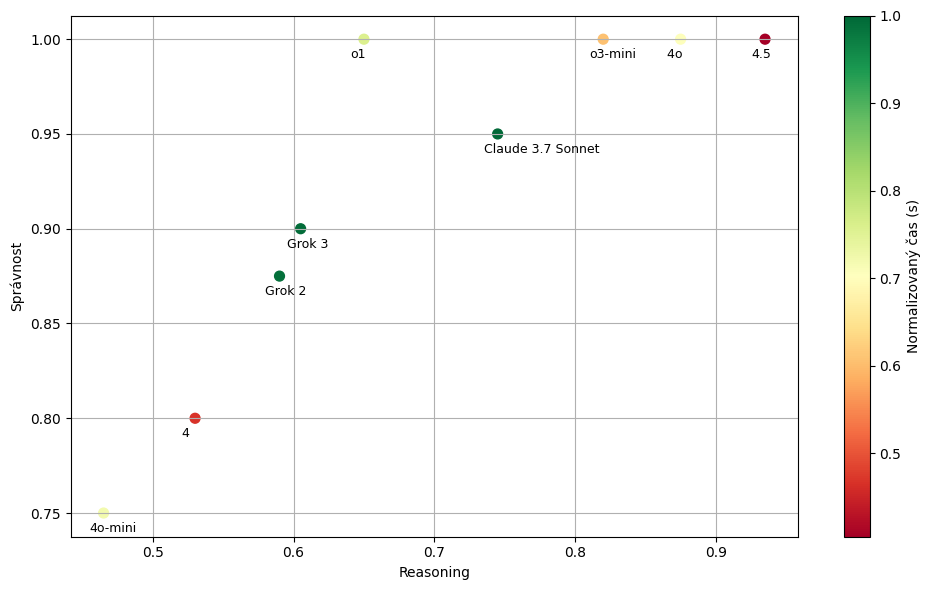
\includegraphics[width=0.8\linewidth]{plot1}
			\caption{Závislost průměrných správnosti odpovědí na komunikačních dovednostech / schopnosti problematiku řádně zpracovat. Zabarvení popisuje rychlost modelu.}
			\label{fig:plot1}
		\end{figure}
		\begin{figure}[H]
			\centering
			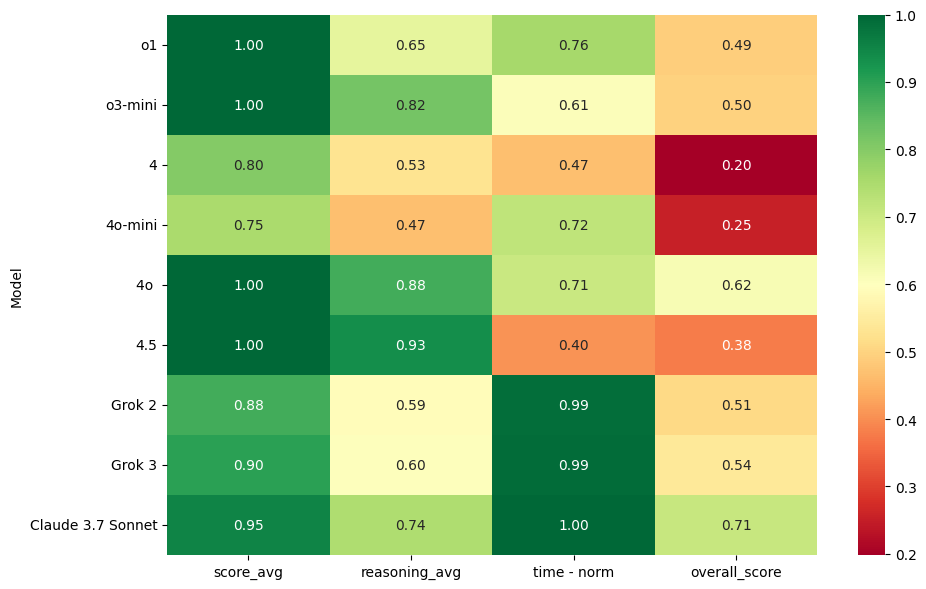
\includegraphics[width=0.8\linewidth]{plot2}
			\caption{Tabulková vizualizace konkrétních průměrných hodnot pro všechny vyšetřované modely.}
			\label{fig:plot2}
		\end{figure}
		Při evaluaci dat pozorujeme, že kombinaci nejvyšší přesnosti a komunikačních dovedností poskytuje ChatGPT 4.5, avšak na úkor času zpracování. Naopak nejhoršími vlastnostmi disponuje model ChatGPT 4 (čemuž se nelze divit, jedná se o starší, neauktuální model). Lze využít způsobu hodnocení a všechny měřené metriky vzájemným vynásobením zkombinovat do jedné, opět platí, že větší hodnoty jsou lepší. Zde se jako naprosto nejhorší ukazuje opět ChatGPT 4, následuje jej 4o-mini a model 4.5 (právě kvůli nejnižší rychlosti zpracování dat). Nejlepší výsledky má v tomto případě Claude 3.7 Sonnet, který dokáže velmi rychle za nízké chybovosti úkoly vyřešit velmi dobře a výstup uživateli srozumitelně prezentovat. Na metrika celkového skóre však nelze pohlížet jako na nejlepší způsob hodnocení, dává totiž všem hodnoceným faktorům stejnou váhu, což nutně nemusí reprezentovat skutečné požadavky - koncový uživatel si kupř. může přát správné a dobře vysvětlené odpovědi, přičemž mu delší čas zpracování odpovědi nutně nemusí vadit.
		
		\section{Zhodnocení výsledků}
		Podařilo se nám modely úspěšně srovnat dle tří důležitých vlastností. Pozorujeme že se všem modelům podařilo materiál předmětu F2050 vyřešit s poměrně nízkou chybovostí, často až tak dobrým způsobem, že by výsledky uživatel mohl pouze přepsat a práci odevzdat jako vlastní (zde je nutno konstatovat, že v tomto předmětu žádné domácí práce nefigurují, tato možnost je tedy zejména hypotetická). \\LLM lze však využít i způsoby méně neetickými - řešení příkladů mohou uživateli značně pomoci pochopit problematiku v předmětu probíranou, zde je zejména velikou výhodou skutečnost, že se lze při potřebě dalšího vysvětlení specifické části řešení modelu jednoduše zeptat, což jiné internetové zdroje (sbírky řešených úloh, videa s přednáškami z jiných univerzit) neumožňují. I zde je však potřeba tuto technologii používat s rozmyslem, zejm. v případě práce s autorskými díly (kupř. materiály z předmětu, které vytvořil sám vyučující). Též je důležité si uvědomit, že výstup jakéhokoliv jazykového modelu (přestože v této práci může mít úspěšnost stoprocentní) může být chybný.  \\
		S uvážením zmíněných rizik mohou být jazykové modely ve studiu užitečné. Předmět F2050 je jedním ze základních kurzů fyziky vyučovaný ve velmi podobné formě na všech fyzikálních oborech na univerzitách po celém světě. Skutečnost, že jazykové modely úspěšně řeší látku v tomto kursu probíranou, implikuje ekvivalentní schopnost zvládnutí problematiky dalších fyzikálních i matematických kursů. Umělá inteligence může být využita smysluplně jako sekundární zdroj pro pochopení probírané látky, ať již to znamená řešení úloh nebo přípravu jinak složitých vizualizací (Obr. 3). Zásadním nedostatkem naší práce absence statistického zpracování dat - výsledky by měly mnohem vyšší kvalitu i výpovědní hodnotu, pokud bychom takto zpracovávali více úloh a nechali modely je zpracovat vícekrát. I přes tento nedostatek však práci hodnotíme jako dostatečný důkaz schopností různých modelů i jejich srovnání.
			\begin{figure}[H]
			\centering
			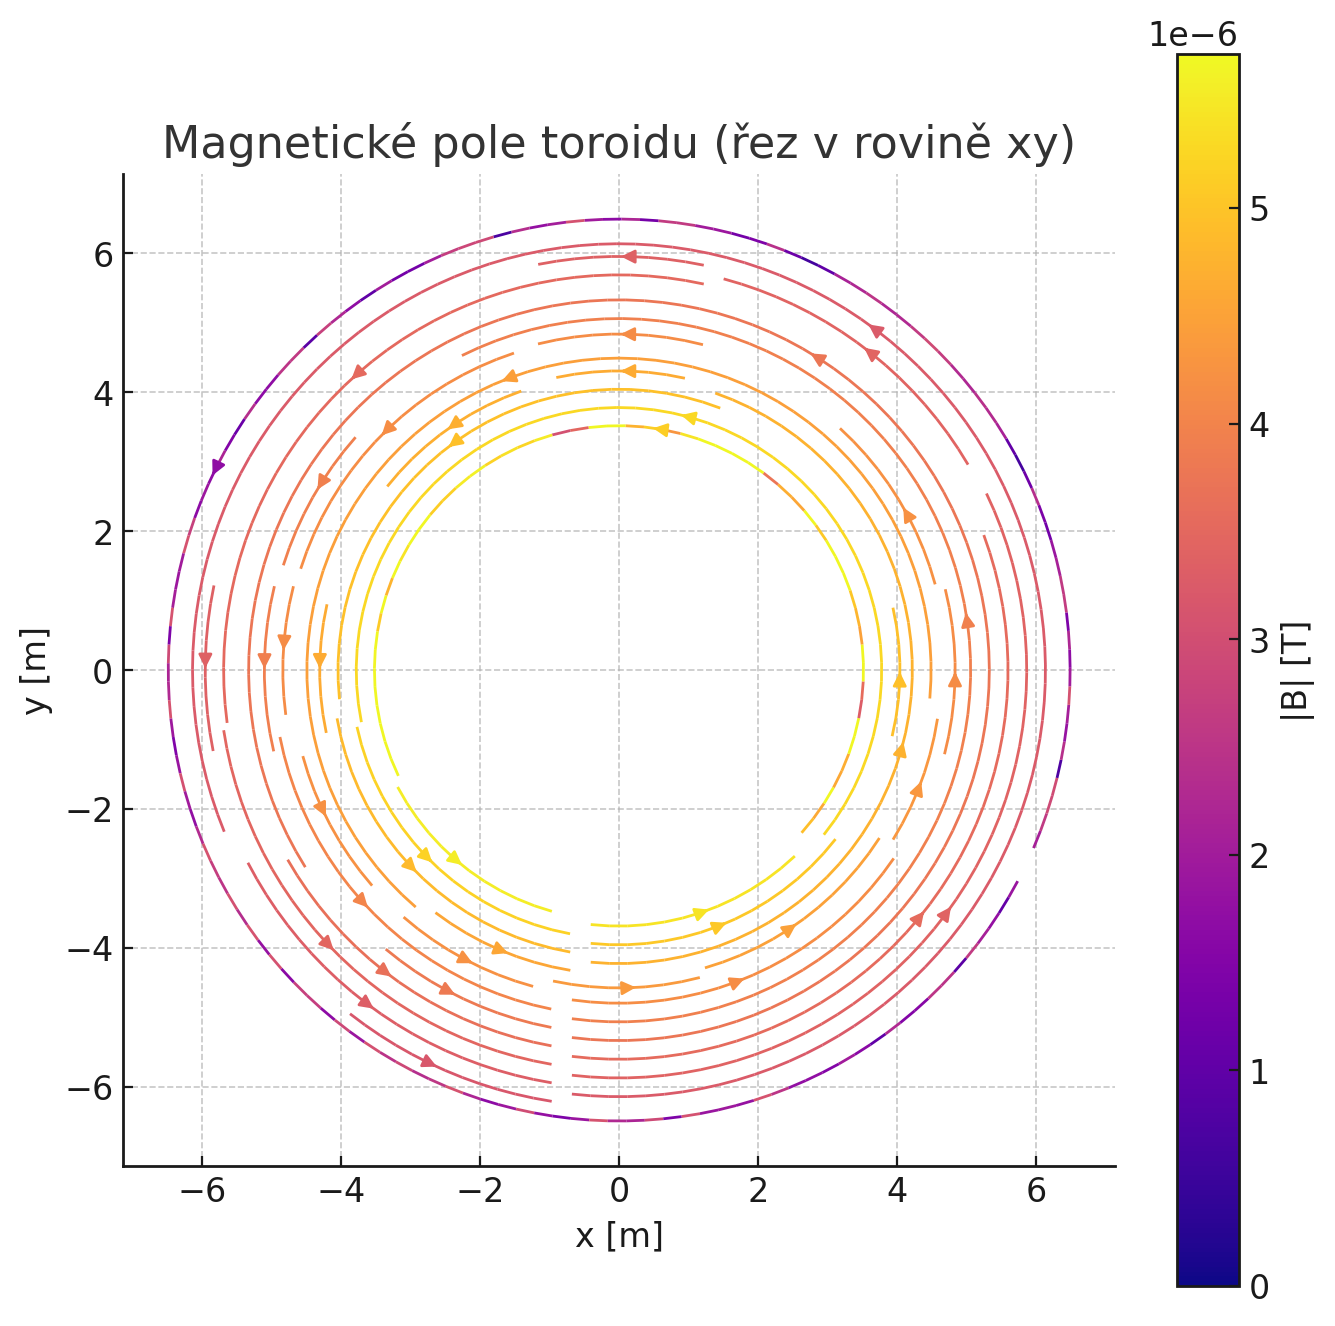
\includegraphics[width=0.8\linewidth]{plot3}
			\caption{Vizualizace magnetického pole toroidu, kód v jazyce Python plně vytvořen ChatGPT, mod. 4o.}
			\label{fig:plot3}
		\end{figure}
		\newpage
		\end{multicols}

	
		
		\section{Zdroje}
		\bibliography{references}
		
		
		
		
		% Nakonec nezapomeňte projet text programem vlna nebo vlnka, např.
		% 	vlna -m -l -n mojeuloha.tex
		% nebo zkontrolovat a opravit jednopísmenné předložky na koncích řádků ručně.

\end{document}
